\section{State of the art image reconstruction}
Long time research.

Major cycle architecture.
Discuss the algorithms 
Split into two parts. We discuss the gridding first. It is responsible

\subsection{Gridding algorithms}
Biggest part is $w$-term, how to handle it efficiently. The WSCLEAN \cite{offringa2014wsclean} did a large part.

More recently, the Image domain gridding algorithm has been developed \cite{veenboer2017image}. Which can put it on the gpu, along with handling more DDE's.

\subsubsection{$w$-stacking}

\subsubsection{Image Domain Gridder}
\begin{figure}[h]
	\centering
	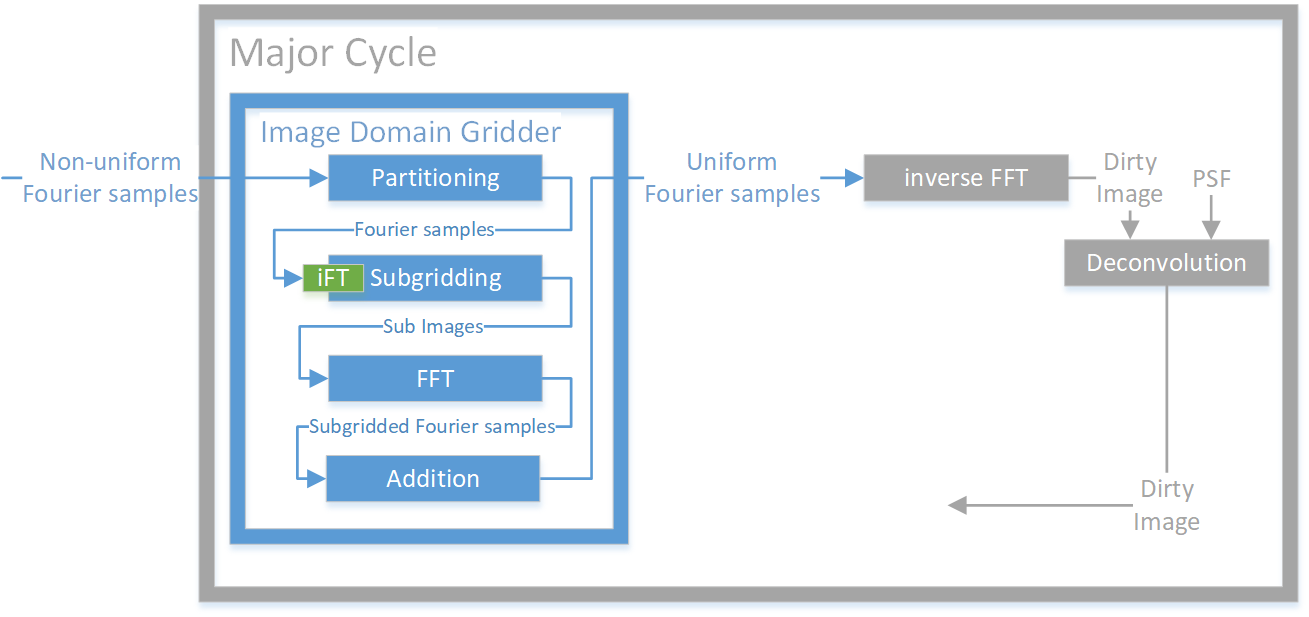
\includegraphics[width=0.80\linewidth]{./chapters/03.distribution/idg/major-minor-idg.png}
	\caption{Image Domain Gridder in the Major Cycle Architecture}
	\label{distribution:idg:system}
\end{figure}

Algorithm
\begin{figure}[h]
	\centering
	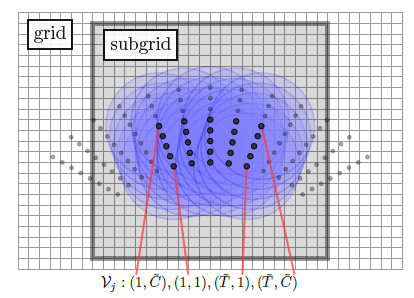
\includegraphics[width=0.40\linewidth]{./chapters/03.distribution/idg/subgrid.png}
	\caption{Subgrid}
	\label{distribution:idg:subgrid}
\end{figure}

\begin{figure}[h]
	\centering
	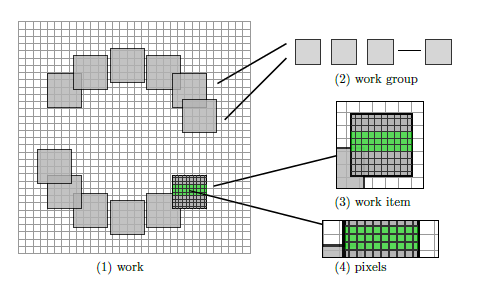
\includegraphics[width=0.40\linewidth]{./chapters/03.distribution/idg/paralellization.png}
	\caption{parallel}
	\label{distribution:idg:parallel}
\end{figure}

\begin{figure}[h]
	\centering
	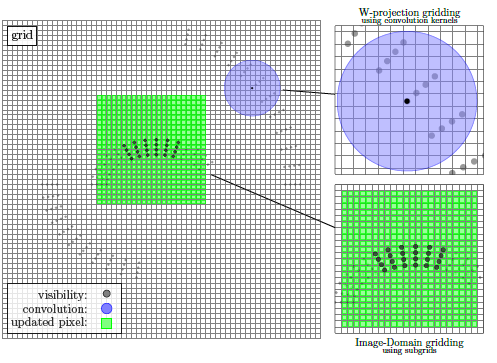
\includegraphics[width=0.40\linewidth]{./chapters/03.distribution/idg/idg0.png}
	\caption{Image Domain Gridder in the Major Cycle Architecture}
	\label{distribution:idg:idg0}
\end{figure}


\subsection{Deconvolution algorithms}
\subsubsection{CLEAN}


\subsection{Reconstruction algorithms which are not based on the deconvolution}
SARA










